\vspace{9em}
\section{Experimental Methodology}
With our evaluation we try to answer: 

1. Can remote storage options keep up with local ones in big data analytic
frameworks.

2. what are the overheads presented with these options.

\note{jk: Make the questions more specific. For example, add a question about
granularity (e.g. 512b and 4KB). So, think carefully what was the evaluation
about and write specific questions. Do not care if they are too much, we are
going to reduce/merge them.}
\vspace{1em}

For the evaluation qe use two servers with Intel Xeon E5-2630 32 Cores @ 2.4
GHz. Each server uses 256GB of DDR4 DRAM divided on two NUMA nodes, each with 16
threads. For storage we use Samsung 970 EVO Plus 2 TB PCIe Gen 3.0 x4 NVMe SSD.
Each server is equipped with Mellanox Technologies ConnectX-3 Network controller
MT27500 with fibre ports compliant with the InfiniBand Architecture
Specification . The servers run CentOS version 7.9 with Linux kernel version is
5.4.267. \note{jk: for tables use latex to create tables and not figures. In the
text when you mention to a Table you say: ``as shown in TableXX'''} Figure 4 shows the server specifications.

\begin{figure}[h]
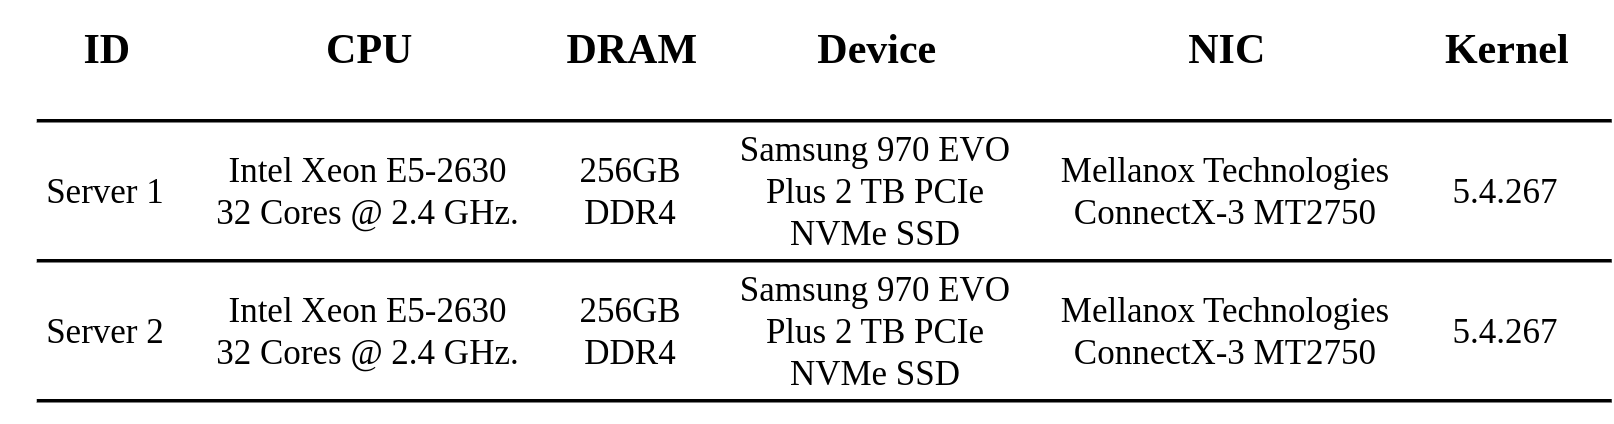
\includegraphics[scale=0.2]{figures/server_specs.drawio.png}\\
\caption{Server specifications table.}
\end{figure}
\vspace{1em}

\textbf{Flexible I/O (FIO) Tester.}
FIO is a widely used open-source tool in the Linux ecosystem for benchmarking
and testing various I/O (input/output) workloads on storage devices. FIO
provides detailed output reports, including metrics such as throughput, IOPS
(input/output operations per second), latency, and CPU utilization. \note{jk: in
the papers we write in present simple} We \note{jk: do not use will} will use
FIO \note{jk: to measure the latency of each different device}
\note{transform the list into table} We will compare accessing latency of each of the following systems: 
\begin{itemize}
    \item Local NVMe drives
    \item Local Ram-disk
    \item Network Block Device (NBD) with NVMe
    \item Network Block Device (NBD) with Ram-disk
    \item Local NVMe drives with SPDK User-Space drivers (User-Space Drive)
    \item Local Ram-disk with SPDK User-Space drivers (User-Space Ram-disk)
    \item NVMe-oF NVMe with SPDK User-Space drivers
    \item NVMe-oF Ram-disk with SPDK User-Space drivers
\end{itemize}
\vspace{1em}

\textbf{Netperf.} 
Netperf is a benchmarking tool used to measure the performance of networking
systems. It's designed to provide a standardized method for measuring networking
performance between two systems. Netperf allows users to test various aspects of
networking performance, such as throughput, latency, and jitter, across
different network protocols like TCP (Transmission Control Protocol) and UDP
(User Datagram Protocol). We will use Netperf to measure end-to-end latency of
TCP (Transmission Control Protocol) To better understand the latency of systems
like Network Block Device (NBD) which uses TCP to export the block device to the
network.
\vspace{1em}

\textbf{TeraHeap} is a system that eliminates S/D overhead and expensive GC scans for a
large portion of the objects in big data frameworks. TeraHeap enhances the
managed runtime environment, particularly the Java Virtual Machine (JVM). It
introduces a supplementary heap, designed for high-capacity storage, alongside
the primary heap. This secondary heap utilizes fast storage and allows direct
access to objects without the need for serialization or deserialization.
Additionally, TeraHeap minimizes the garbage collection overhead by preventing
the garbage collector from scanning the secondary heap. It takes advantage of
frameworks' capability to designate certain objects for off-heap allocation and
provides them with a hint-based method for relocating these objects to the
secondary heap. We will use Teraheap as a Real world system. We configure Teraheap to apply the supplementary heap to local and remote block devices and compare the performances of each block device system.
\vspace{1em}

\textbf{Tasks, datasets and Execution time breakdown:} We employ eight memory-intensive tasks from Spark-Bench and five LDBC Graphalytics suites for Giraph, generating datasets accordingly. Each experiment is run five times, and the average end-to-end execution time is recorded. Time breakdown includes 'other' time, S/D plus I/O time, minor GC time, and major GC time. 'Other' time covers mutator threads, potentially including I/O wait. The profiler operates with minimal overhead. We configure TeraHeap to allocate the first heap (H1) on DRAM and the second heap (H2) over a file in Local or Remote block device via memory-mapped I/O (mmio) we also limmit DRAM and H1 to a fixed size to create pressure and more I/O to H2. Figure 5 shows the DRAM and H1 size in each workload, in Spark and Giraph, accordingly.
\begin{figure}[h]
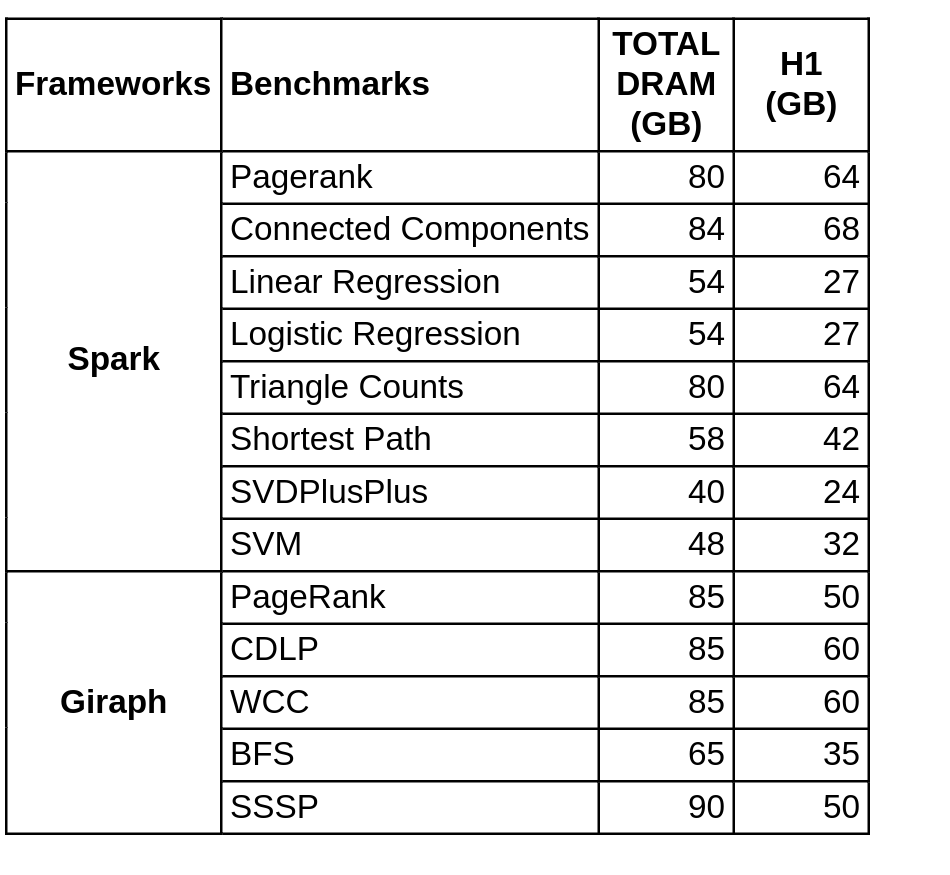
\includegraphics[scale=0.2]{figures/tera_task_conf.drawio.png}\\
\caption{Teraheap workload Configurations of Giraph and Spark.}
\end{figure}

\begin{itemize}
    \item explain the environment. server infrastructure kernel nvmes ....
    \item talk about FIO 
    \item talk about netperf and how it can show stats of TCP lattency
    \item talk about the setups of microbenchmarks and how we will use them to break down the lattencies
    \item talk about Teraheap and the way it uses a second heap over block device
    \item talk about teraheap benchmarks
\end{itemize}
